\chapter{Detecting equivalences}

Sheer throughput might not be sufficient to perform a full Platypus
tournament in a reasonable time frame. Even if we could run one billion
matches per second, we would still require approximately 2.3 years to run
all $2^{56}$ matches in the full tournament.

Baker \cite{triangle} discusses the optimisation of a brute force problem,
which makes many calls to a pure function with the same arguments.
He notes that \emph{memoisation} -- caching the results of an
expensive function call instead of recomputing the results -- allows
``one processor [to simulate] the execution of many processes with a single
execution''. But we never run a game between the exact same machines
more than once, so memoisation per se would not be effective.

We could still use the same principle if we could detect machines
which are \emph{equivalent} in a more abstract sense: two machines
are equivalent if they behave identically when faced against the same
opponent. We may then use knowledge of such equivalence to reduce the
number of matches played: the results of a match between machines $m_1$ and
$m_2$ must be identical to the results of a match between machines $m_3$
and $m_2$ if $m_1$ and $m_3$ are equivalent.
Exploiting such equivalences can provide a substantial speedup as the Platypus
tournament plays every machine against every machine, so reducing the
number of machines by some factor $f$ reduces the number of necessary
games to play by a factor $f^2$.

All the algorithms are implemented in the file \texttt{Code/equivalences.lisp}.
Generation of diagrams is implemented in the file \texttt{Code/report-diagrams.lisp}.

\section{Dead code elimination}

Consider the machines depicted in Figure~\ref{fig:dead-states}.
Both machines always move towards the ghost gum and turn
all cells Yellow, and thus the machines are equivalent, despite
five of the seven transitions being different. Any
configuration of these five transitions cannot affect the behaviour
of the machine, as there is no way for the machine to perform
these transitions. There are $(2^4)^5 = 1048576$ machines in total
which are equivalent to either machine, and we would prefer
to avoid running matches involving all of these machines. We
may use a \emph{dead code elimination} algorithm to normalise
all these machines to just one machine.

\begin{figure}
  \begin{center}
    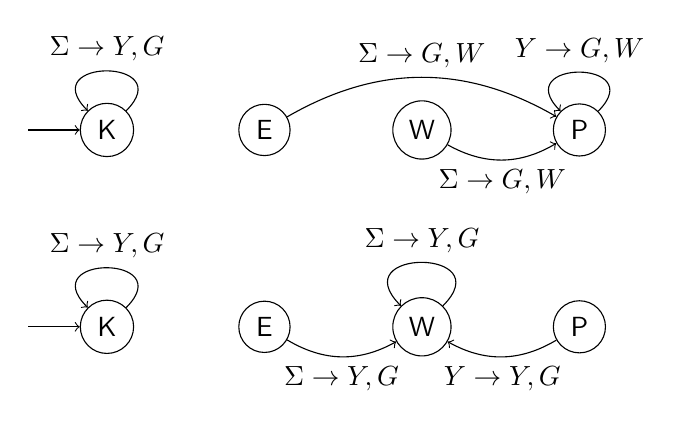
\begin{tikzpicture}
      \node[draw, circle] (P1) at (6, 0) {\sffamily P};
      \node[draw, circle] (W1) at (4, 0) {\sffamily W};
      \node[draw, circle] (E1) at (2, 0) {\sffamily E};
      \node[draw, circle] (K1) at (0, 0) {\sffamily K};
      \draw[->] (-1, 0) to (K1);
      \draw[->] (P1) to[in=135, out=45, looseness=5] node[midway, above] {$\q{Y} \rightarrow \q{G}, \q{W}$} (P1);
      \draw[->] (W1) to[bend right] node[midway, below] {$\Sigma \rightarrow \q{G}, \q{W}$} (P1);
      \draw[->] (E1) to[bend left] node[midway, above] {$\Sigma \rightarrow \q{G}, \q{W}$} (P1);
      \draw[->] (K1) to[in=135, out=45, looseness=5] node[midway, above] {$\Sigma \rightarrow \q{Y}, \q{G}$} (K1);
    
      \node[draw, circle] (P2) at (6, -2.5) {\sffamily P};
      \node[draw, circle] (W2) at (4, -2.5) {\sffamily W};
      \node[draw, circle] (E2) at (2, -2.5) {\sffamily E};
      \node[draw, circle] (K2) at (0, -2.5) {\sffamily K};
      \draw[->] (-1, -2.5) to (K2);
      \draw[->] (P2) to[bend left] node[midway, below] {$\q{Y} \rightarrow \q{Y}, \q{G}$} (W2);
      \draw[->] (W2) to[in=135, out=45, looseness=5] node[midway, above] {$\Sigma \rightarrow \q{Y}, \q{G}$} (W2);
      \draw[->] (E2) to[bend right] node[midway, below] {$\Sigma \rightarrow \q{Y}, \q{G}$} (W2);
      \draw[->] (K2) to[in=135, out=45, looseness=5] node[midway, above] {$\Sigma \rightarrow \q{Y}, \q{G}$} (K2);
    \end{tikzpicture}
  \end{center}
  \caption{Two equivalent machines (\texttt{\#xFF00000} and \texttt{\#xFFBBBBB}).}
  \label{fig:dead-states}
\end{figure}

A state is considered \emph{live} if it is either the initial state
state (the Kangaroo state in the Platypus game), or can be entered by
transitioning from another live state. All other states are \emph{dead}.
The transitions from a dead state cannot influence the behaviour
of a Platypus machine, as the machine cannot possibly transition
to a dead state. I traverse the transitions of the machine starting from
the Kangaroo state and copy transitions to another machine, leaving
all the transitions from unreachable states unset. 

108,988,816 unique machines (40.6\%) remain after dead code elimination.
The results are presented as a heatmap of unique machines after
deduplication in Figure~\ref{fig:dce}, with the X and Y axes having
different animals to transition to from the Kangaroo and Emu
states respectively. Almost no machines with only the Kangaroo state
live (the white stripe on the right) or only just the Kangaroo and
Emu states live remain. It took 109 CPU-seconds to eliminate
dead code from every Platypus machine.


\begin{figure}
  \begin{center}
    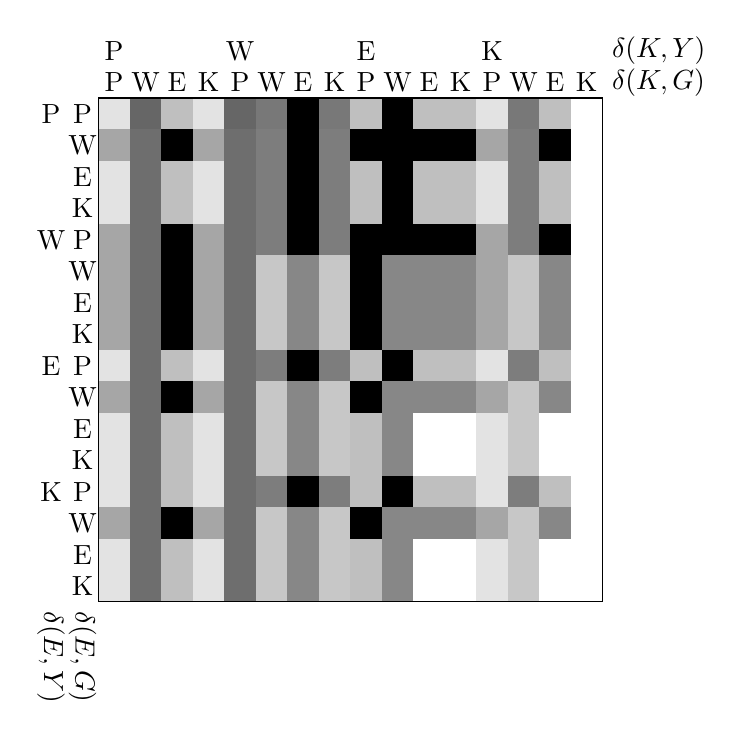
\begin{tikzpicture}[yscale=-1, scale=0.4]
  \node[anchor=west] at (16, -1.5) {$\delta (\q{K}, \q{Y})$};
  \node[anchor=west] at (16, -0.5) {$\delta (\q{K}, \q{G})$};
  \node[anchor=west, rotate=-90] at (-1.5, 16) {$\delta (\q{E}, \q{Y})$};
  \node[anchor=west, rotate=-90] at (-0.5, 16) {$\delta (\q{E}, \q{G})$};
  \node at (0.5, -1.5) {P}; \node at (-1.5, 0.5) {P};
  \node at (0.5, -0.5) {P}; \node at (-0.5, 0.5) {P};
  \node at (4.5, -0.5) {P}; \node at (-0.5, 4.5) {P};
  \node at (8.5, -0.5) {P}; \node at (-0.5, 8.5) {P};
  \node at (12.5, -0.5) {P}; \node at (-0.5, 12.5) {P};
  \node at (4.5, -1.5) {W}; \node at (-1.5, 4.5) {W};
  \node at (1.5, -0.5) {W}; \node at (-0.5, 1.5) {W};
  \node at (5.5, -0.5) {W}; \node at (-0.5, 5.5) {W};
  \node at (9.5, -0.5) {W}; \node at (-0.5, 9.5) {W};
  \node at (13.5, -0.5) {W}; \node at (-0.5, 13.5) {W};
  \node at (8.5, -1.5) {E}; \node at (-1.5, 8.5) {E};
  \node at (2.5, -0.5) {E}; \node at (-0.5, 2.5) {E};
  \node at (6.5, -0.5) {E}; \node at (-0.5, 6.5) {E};
  \node at (10.5, -0.5) {E}; \node at (-0.5, 10.5) {E};
  \node at (14.5, -0.5) {E}; \node at (-0.5, 14.5) {E};
  \node at (12.5, -1.5) {K}; \node at (-1.5, 12.5) {K};
  \node at (3.5, -0.5) {K}; \node at (-0.5, 3.5) {K};
  \node at (7.5, -0.5) {K}; \node at (-0.5, 7.5) {K};
  \node at (11.5, -0.5) {K}; \node at (-0.5, 11.5) {K};
  \node at (15.5, -0.5) {K}; \node at (-0.5, 15.5) {K};
  \fill[black!11!white] (0, 0) rectangle +(1, 1);
  \fill[black!35!white] (0, 1) rectangle +(1, 1);
  \fill[black!11!white] (0, 2) rectangle +(1, 1);
  \fill[black!11!white] (0, 3) rectangle +(1, 1);
  \fill[black!35!white] (0, 4) rectangle +(1, 1);
  \fill[black!35!white] (0, 5) rectangle +(1, 1);
  \fill[black!35!white] (0, 6) rectangle +(1, 1);
  \fill[black!35!white] (0, 7) rectangle +(1, 1);
  \fill[black!11!white] (0, 8) rectangle +(1, 1);
  \fill[black!35!white] (0, 9) rectangle +(1, 1);
  \fill[black!11!white] (0, 10) rectangle +(1, 1);
  \fill[black!11!white] (0, 11) rectangle +(1, 1);
  \fill[black!11!white] (0, 12) rectangle +(1, 1);
  \fill[black!35!white] (0, 13) rectangle +(1, 1);
  \fill[black!11!white] (0, 14) rectangle +(1, 1);
  \fill[black!11!white] (0, 15) rectangle +(1, 1);
  \fill[black!60!white] (1, 0) rectangle +(1, 1);
  \fill[black!57!white] (1, 1) rectangle +(1, 1);
  \fill[black!57!white] (1, 2) rectangle +(1, 1);
  \fill[black!57!white] (1, 3) rectangle +(1, 1);
  \fill[black!57!white] (1, 4) rectangle +(1, 1);
  \fill[black!57!white] (1, 5) rectangle +(1, 1);
  \fill[black!57!white] (1, 6) rectangle +(1, 1);
  \fill[black!57!white] (1, 7) rectangle +(1, 1);
  \fill[black!57!white] (1, 8) rectangle +(1, 1);
  \fill[black!57!white] (1, 9) rectangle +(1, 1);
  \fill[black!57!white] (1, 10) rectangle +(1, 1);
  \fill[black!57!white] (1, 11) rectangle +(1, 1);
  \fill[black!57!white] (1, 12) rectangle +(1, 1);
  \fill[black!57!white] (1, 13) rectangle +(1, 1);
  \fill[black!57!white] (1, 14) rectangle +(1, 1);
  \fill[black!57!white] (1, 15) rectangle +(1, 1);
  \fill[black!25!white] (2, 0) rectangle +(1, 1);
  \fill[black!100!white] (2, 1) rectangle +(1, 1);
  \fill[black!25!white] (2, 2) rectangle +(1, 1);
  \fill[black!25!white] (2, 3) rectangle +(1, 1);
  \fill[black!100!white] (2, 4) rectangle +(1, 1);
  \fill[black!100!white] (2, 5) rectangle +(1, 1);
  \fill[black!100!white] (2, 6) rectangle +(1, 1);
  \fill[black!100!white] (2, 7) rectangle +(1, 1);
  \fill[black!25!white] (2, 8) rectangle +(1, 1);
  \fill[black!100!white] (2, 9) rectangle +(1, 1);
  \fill[black!25!white] (2, 10) rectangle +(1, 1);
  \fill[black!25!white] (2, 11) rectangle +(1, 1);
  \fill[black!25!white] (2, 12) rectangle +(1, 1);
  \fill[black!100!white] (2, 13) rectangle +(1, 1);
  \fill[black!25!white] (2, 14) rectangle +(1, 1);
  \fill[black!25!white] (2, 15) rectangle +(1, 1);
  \fill[black!11!white] (3, 0) rectangle +(1, 1);
  \fill[black!35!white] (3, 1) rectangle +(1, 1);
  \fill[black!11!white] (3, 2) rectangle +(1, 1);
  \fill[black!11!white] (3, 3) rectangle +(1, 1);
  \fill[black!35!white] (3, 4) rectangle +(1, 1);
  \fill[black!35!white] (3, 5) rectangle +(1, 1);
  \fill[black!35!white] (3, 6) rectangle +(1, 1);
  \fill[black!35!white] (3, 7) rectangle +(1, 1);
  \fill[black!11!white] (3, 8) rectangle +(1, 1);
  \fill[black!35!white] (3, 9) rectangle +(1, 1);
  \fill[black!11!white] (3, 10) rectangle +(1, 1);
  \fill[black!11!white] (3, 11) rectangle +(1, 1);
  \fill[black!11!white] (3, 12) rectangle +(1, 1);
  \fill[black!35!white] (3, 13) rectangle +(1, 1);
  \fill[black!11!white] (3, 14) rectangle +(1, 1);
  \fill[black!11!white] (3, 15) rectangle +(1, 1);
  \fill[black!60!white] (4, 0) rectangle +(1, 1);
  \fill[black!57!white] (4, 1) rectangle +(1, 1);
  \fill[black!57!white] (4, 2) rectangle +(1, 1);
  \fill[black!57!white] (4, 3) rectangle +(1, 1);
  \fill[black!57!white] (4, 4) rectangle +(1, 1);
  \fill[black!57!white] (4, 5) rectangle +(1, 1);
  \fill[black!57!white] (4, 6) rectangle +(1, 1);
  \fill[black!57!white] (4, 7) rectangle +(1, 1);
  \fill[black!57!white] (4, 8) rectangle +(1, 1);
  \fill[black!57!white] (4, 9) rectangle +(1, 1);
  \fill[black!57!white] (4, 10) rectangle +(1, 1);
  \fill[black!57!white] (4, 11) rectangle +(1, 1);
  \fill[black!57!white] (4, 12) rectangle +(1, 1);
  \fill[black!57!white] (4, 13) rectangle +(1, 1);
  \fill[black!57!white] (4, 14) rectangle +(1, 1);
  \fill[black!57!white] (4, 15) rectangle +(1, 1);
  \fill[black!53!white] (5, 0) rectangle +(1, 1);
  \fill[black!51!white] (5, 1) rectangle +(1, 1);
  \fill[black!51!white] (5, 2) rectangle +(1, 1);
  \fill[black!51!white] (5, 3) rectangle +(1, 1);
  \fill[black!51!white] (5, 4) rectangle +(1, 1);
  \fill[black!22!white] (5, 5) rectangle +(1, 1);
  \fill[black!22!white] (5, 6) rectangle +(1, 1);
  \fill[black!22!white] (5, 7) rectangle +(1, 1);
  \fill[black!51!white] (5, 8) rectangle +(1, 1);
  \fill[black!22!white] (5, 9) rectangle +(1, 1);
  \fill[black!22!white] (5, 10) rectangle +(1, 1);
  \fill[black!22!white] (5, 11) rectangle +(1, 1);
  \fill[black!51!white] (5, 12) rectangle +(1, 1);
  \fill[black!22!white] (5, 13) rectangle +(1, 1);
  \fill[black!22!white] (5, 14) rectangle +(1, 1);
  \fill[black!22!white] (5, 15) rectangle +(1, 1);
  \fill[black!100!white] (6, 0) rectangle +(1, 1);
  \fill[black!100!white] (6, 1) rectangle +(1, 1);
  \fill[black!100!white] (6, 2) rectangle +(1, 1);
  \fill[black!100!white] (6, 3) rectangle +(1, 1);
  \fill[black!100!white] (6, 4) rectangle +(1, 1);
  \fill[black!47!white] (6, 5) rectangle +(1, 1);
  \fill[black!47!white] (6, 6) rectangle +(1, 1);
  \fill[black!47!white] (6, 7) rectangle +(1, 1);
  \fill[black!100!white] (6, 8) rectangle +(1, 1);
  \fill[black!47!white] (6, 9) rectangle +(1, 1);
  \fill[black!47!white] (6, 10) rectangle +(1, 1);
  \fill[black!47!white] (6, 11) rectangle +(1, 1);
  \fill[black!100!white] (6, 12) rectangle +(1, 1);
  \fill[black!47!white] (6, 13) rectangle +(1, 1);
  \fill[black!47!white] (6, 14) rectangle +(1, 1);
  \fill[black!47!white] (6, 15) rectangle +(1, 1);
  \fill[black!53!white] (7, 0) rectangle +(1, 1);
  \fill[black!51!white] (7, 1) rectangle +(1, 1);
  \fill[black!51!white] (7, 2) rectangle +(1, 1);
  \fill[black!51!white] (7, 3) rectangle +(1, 1);
  \fill[black!51!white] (7, 4) rectangle +(1, 1);
  \fill[black!22!white] (7, 5) rectangle +(1, 1);
  \fill[black!22!white] (7, 6) rectangle +(1, 1);
  \fill[black!22!white] (7, 7) rectangle +(1, 1);
  \fill[black!51!white] (7, 8) rectangle +(1, 1);
  \fill[black!22!white] (7, 9) rectangle +(1, 1);
  \fill[black!22!white] (7, 10) rectangle +(1, 1);
  \fill[black!22!white] (7, 11) rectangle +(1, 1);
  \fill[black!51!white] (7, 12) rectangle +(1, 1);
  \fill[black!22!white] (7, 13) rectangle +(1, 1);
  \fill[black!22!white] (7, 14) rectangle +(1, 1);
  \fill[black!22!white] (7, 15) rectangle +(1, 1);
  \fill[black!25!white] (8, 0) rectangle +(1, 1);
  \fill[black!100!white] (8, 1) rectangle +(1, 1);
  \fill[black!25!white] (8, 2) rectangle +(1, 1);
  \fill[black!25!white] (8, 3) rectangle +(1, 1);
  \fill[black!100!white] (8, 4) rectangle +(1, 1);
  \fill[black!100!white] (8, 5) rectangle +(1, 1);
  \fill[black!100!white] (8, 6) rectangle +(1, 1);
  \fill[black!100!white] (8, 7) rectangle +(1, 1);
  \fill[black!25!white] (8, 8) rectangle +(1, 1);
  \fill[black!100!white] (8, 9) rectangle +(1, 1);
  \fill[black!25!white] (8, 10) rectangle +(1, 1);
  \fill[black!25!white] (8, 11) rectangle +(1, 1);
  \fill[black!25!white] (8, 12) rectangle +(1, 1);
  \fill[black!100!white] (8, 13) rectangle +(1, 1);
  \fill[black!25!white] (8, 14) rectangle +(1, 1);
  \fill[black!25!white] (8, 15) rectangle +(1, 1);
  \fill[black!100!white] (9, 0) rectangle +(1, 1);
  \fill[black!100!white] (9, 1) rectangle +(1, 1);
  \fill[black!100!white] (9, 2) rectangle +(1, 1);
  \fill[black!100!white] (9, 3) rectangle +(1, 1);
  \fill[black!100!white] (9, 4) rectangle +(1, 1);
  \fill[black!47!white] (9, 5) rectangle +(1, 1);
  \fill[black!47!white] (9, 6) rectangle +(1, 1);
  \fill[black!47!white] (9, 7) rectangle +(1, 1);
  \fill[black!100!white] (9, 8) rectangle +(1, 1);
  \fill[black!47!white] (9, 9) rectangle +(1, 1);
  \fill[black!47!white] (9, 10) rectangle +(1, 1);
  \fill[black!47!white] (9, 11) rectangle +(1, 1);
  \fill[black!100!white] (9, 12) rectangle +(1, 1);
  \fill[black!47!white] (9, 13) rectangle +(1, 1);
  \fill[black!47!white] (9, 14) rectangle +(1, 1);
  \fill[black!47!white] (9, 15) rectangle +(1, 1);
  \fill[black!25!white] (10, 0) rectangle +(1, 1);
  \fill[black!100!white] (10, 1) rectangle +(1, 1);
  \fill[black!25!white] (10, 2) rectangle +(1, 1);
  \fill[black!25!white] (10, 3) rectangle +(1, 1);
  \fill[black!100!white] (10, 4) rectangle +(1, 1);
  \fill[black!47!white] (10, 5) rectangle +(1, 1);
  \fill[black!47!white] (10, 6) rectangle +(1, 1);
  \fill[black!47!white] (10, 7) rectangle +(1, 1);
  \fill[black!25!white] (10, 8) rectangle +(1, 1);
  \fill[black!47!white] (10, 9) rectangle +(1, 1);
  \fill[black!0!white] (10, 10) rectangle +(1, 1);
  \fill[black!0!white] (10, 11) rectangle +(1, 1);
  \fill[black!25!white] (10, 12) rectangle +(1, 1);
  \fill[black!47!white] (10, 13) rectangle +(1, 1);
  \fill[black!0!white] (10, 14) rectangle +(1, 1);
  \fill[black!0!white] (10, 15) rectangle +(1, 1);
  \fill[black!25!white] (11, 0) rectangle +(1, 1);
  \fill[black!100!white] (11, 1) rectangle +(1, 1);
  \fill[black!25!white] (11, 2) rectangle +(1, 1);
  \fill[black!25!white] (11, 3) rectangle +(1, 1);
  \fill[black!100!white] (11, 4) rectangle +(1, 1);
  \fill[black!47!white] (11, 5) rectangle +(1, 1);
  \fill[black!47!white] (11, 6) rectangle +(1, 1);
  \fill[black!47!white] (11, 7) rectangle +(1, 1);
  \fill[black!25!white] (11, 8) rectangle +(1, 1);
  \fill[black!47!white] (11, 9) rectangle +(1, 1);
  \fill[black!0!white] (11, 10) rectangle +(1, 1);
  \fill[black!0!white] (11, 11) rectangle +(1, 1);
  \fill[black!25!white] (11, 12) rectangle +(1, 1);
  \fill[black!47!white] (11, 13) rectangle +(1, 1);
  \fill[black!0!white] (11, 14) rectangle +(1, 1);
  \fill[black!0!white] (11, 15) rectangle +(1, 1);
  \fill[black!11!white] (12, 0) rectangle +(1, 1);
  \fill[black!35!white] (12, 1) rectangle +(1, 1);
  \fill[black!11!white] (12, 2) rectangle +(1, 1);
  \fill[black!11!white] (12, 3) rectangle +(1, 1);
  \fill[black!35!white] (12, 4) rectangle +(1, 1);
  \fill[black!35!white] (12, 5) rectangle +(1, 1);
  \fill[black!35!white] (12, 6) rectangle +(1, 1);
  \fill[black!35!white] (12, 7) rectangle +(1, 1);
  \fill[black!11!white] (12, 8) rectangle +(1, 1);
  \fill[black!35!white] (12, 9) rectangle +(1, 1);
  \fill[black!11!white] (12, 10) rectangle +(1, 1);
  \fill[black!11!white] (12, 11) rectangle +(1, 1);
  \fill[black!11!white] (12, 12) rectangle +(1, 1);
  \fill[black!35!white] (12, 13) rectangle +(1, 1);
  \fill[black!11!white] (12, 14) rectangle +(1, 1);
  \fill[black!11!white] (12, 15) rectangle +(1, 1);
  \fill[black!53!white] (13, 0) rectangle +(1, 1);
  \fill[black!51!white] (13, 1) rectangle +(1, 1);
  \fill[black!51!white] (13, 2) rectangle +(1, 1);
  \fill[black!51!white] (13, 3) rectangle +(1, 1);
  \fill[black!51!white] (13, 4) rectangle +(1, 1);
  \fill[black!22!white] (13, 5) rectangle +(1, 1);
  \fill[black!22!white] (13, 6) rectangle +(1, 1);
  \fill[black!22!white] (13, 7) rectangle +(1, 1);
  \fill[black!51!white] (13, 8) rectangle +(1, 1);
  \fill[black!22!white] (13, 9) rectangle +(1, 1);
  \fill[black!22!white] (13, 10) rectangle +(1, 1);
  \fill[black!22!white] (13, 11) rectangle +(1, 1);
  \fill[black!51!white] (13, 12) rectangle +(1, 1);
  \fill[black!22!white] (13, 13) rectangle +(1, 1);
  \fill[black!22!white] (13, 14) rectangle +(1, 1);
  \fill[black!22!white] (13, 15) rectangle +(1, 1);
  \fill[black!25!white] (14, 0) rectangle +(1, 1);
  \fill[black!100!white] (14, 1) rectangle +(1, 1);
  \fill[black!25!white] (14, 2) rectangle +(1, 1);
  \fill[black!25!white] (14, 3) rectangle +(1, 1);
  \fill[black!100!white] (14, 4) rectangle +(1, 1);
  \fill[black!47!white] (14, 5) rectangle +(1, 1);
  \fill[black!47!white] (14, 6) rectangle +(1, 1);
  \fill[black!47!white] (14, 7) rectangle +(1, 1);
  \fill[black!25!white] (14, 8) rectangle +(1, 1);
  \fill[black!47!white] (14, 9) rectangle +(1, 1);
  \fill[black!0!white] (14, 10) rectangle +(1, 1);
  \fill[black!0!white] (14, 11) rectangle +(1, 1);
  \fill[black!25!white] (14, 12) rectangle +(1, 1);
  \fill[black!47!white] (14, 13) rectangle +(1, 1);
  \fill[black!0!white] (14, 14) rectangle +(1, 1);
  \fill[black!0!white] (14, 15) rectangle +(1, 1);
  \fill[black!0!white] (15, 0) rectangle +(1, 1);
  \fill[black!0!white] (15, 1) rectangle +(1, 1);
  \fill[black!0!white] (15, 2) rectangle +(1, 1);
  \fill[black!0!white] (15, 3) rectangle +(1, 1);
  \fill[black!0!white] (15, 4) rectangle +(1, 1);
  \fill[black!0!white] (15, 5) rectangle +(1, 1);
  \fill[black!0!white] (15, 6) rectangle +(1, 1);
  \fill[black!0!white] (15, 7) rectangle +(1, 1);
  \fill[black!0!white] (15, 8) rectangle +(1, 1);
  \fill[black!0!white] (15, 9) rectangle +(1, 1);
  \fill[black!0!white] (15, 10) rectangle +(1, 1);
  \fill[black!0!white] (15, 11) rectangle +(1, 1);
  \fill[black!0!white] (15, 12) rectangle +(1, 1);
  \fill[black!0!white] (15, 13) rectangle +(1, 1);
  \fill[black!0!white] (15, 14) rectangle +(1, 1);
  \fill[black!0!white] (15, 15) rectangle +(1, 1);
  \draw (0, 0) rectangle (16, 16);
\end{tikzpicture}
  \end{center}
  \caption{A heatmap of the distribution of unique machines after dead code elimination. Darker squares have more machines.}
  \label{fig:dce}
\end{figure}

\section{Renaming}

Now consider the machines depicted in Figure~\ref{fig:renaming-states}.
The machines are equivalent, as one may be obtained from the other
by swapping the Emu and Wombat states. (Note that the Emu and
Wombat states were rearranged, in order to make the identical
structure of the machines more apparent.) All machines which have
live Emu and Wombat states thus have a different \emph{mirror image},
which dead code elimination cannot detect; but we may also detect
mirror images with another algorithm.

\begin{figure}
  \begin{center}
    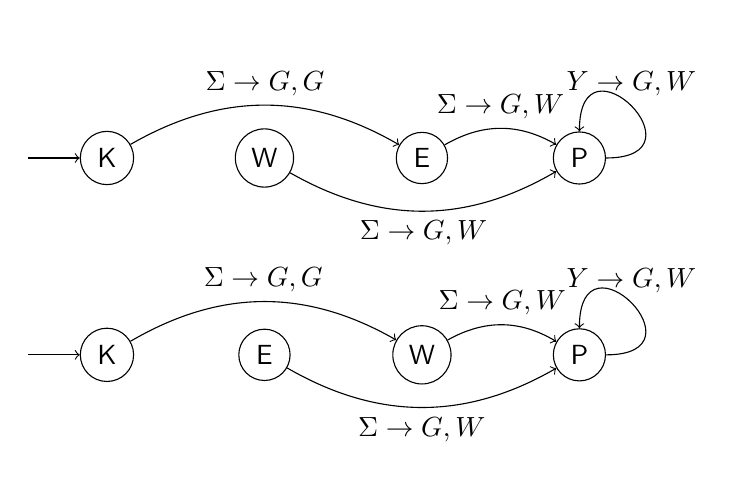
\begin{tikzpicture}
      \node[draw, circle] (P1) at (6, 0) {\sffamily P};
      \node[draw, circle] (W1) at (4, 0) {\sffamily W};
      \node[draw, circle] (E1) at (2, 0) {\sffamily E};
      \node[draw, circle] (K1) at (0, 0) {\sffamily K};
      \draw[->] (-1, 0) to (K1);
      \draw[->] (P1) to[in=90, out=0, looseness=7] node[midway, above] {$\q{Y} \rightarrow \q{G}, \q{W}$} (P1);
      \draw[->] (W1) to[bend left] node[midway, above] {$\Sigma \rightarrow \q{G}, \q{W}$} (P1);
      \draw[->] (E1) to[bend right] node[midway, below] {$\Sigma \rightarrow \q{G}, \q{W}$} (P1);
      \draw[->] (K1) to[bend left] node[midway, above] {$\Sigma \rightarrow \q{G}, \q{G}$} (W1);
      
      \node[draw, circle] (P2) at (6, 2.5) {\sffamily P};
      \node[draw, circle] (W2) at (2, 2.5) {\sffamily W};
      \node[draw, circle] (E2) at (4, 2.5) {\sffamily E};
      \node[draw, circle] (K2) at (0, 2.5) {\sffamily K};
      \draw[->] (-1, 2.5) to (K2);
      \draw[->] (P2) to[in=90, out=0, looseness=7] node[midway, above] {$\q{Y} \rightarrow \q{G}, \q{W}$} (P2);
      \draw[->] (W2) to[bend right] node[midway, below] {$\Sigma \rightarrow \q{G}, \q{W}$} (P2);
      \draw[->] (E2) to[bend left] node[midway, above] {$\Sigma \rightarrow \q{G}, \q{W}$} (P2);
      \draw[->] (K2) to[bend left] node[midway, above] {$\Sigma \rightarrow \q{G}, \q{G}$} (E2);
    \end{tikzpicture}
  \end{center}
  \caption{Two equivalent machines (\texttt{\#xAA00000} and \texttt{\#xCC00000}).}
  \label{fig:renaming-states}
\end{figure}

Two Turing machines $M_1$ and $M_2$ are identical if $M_2$
can be produced by renaming states in $M_1$. The Emu
and Wombat states may be swapped in a Platypus machine; but the
Kangaroo and Platypus states cannot be swapped with other states,
as the Kangaroo state is always the initial state, and the Platypus
state always is missing a transition.

A traversal of the machine can be used to normalise a mirror image,
mapping the first state other than Kangaroo or Platypus encountered
to the Emu state. I use a depth-first traversal, visiting the transition
on reading Yellow first, though the particular traversal used does not
affect efficacy. The traversal builds a new machine with the mapping
applied. However, it could be possible that both the Emu and Wombat
states are dead, so no assignment is possible; this algorithm does
not ever insert transitions from dead states, implicitly performing
dead-code elimination, and so the mapping does not matter.

54,494,608 unique machines (20.3\%) remain after renaming states.
This figure is very close to half the machines remaining after
dead code elimination, but 200 machines do not have live Emu or
Wombat states, and so cannot be normalised. The results are
presented in Figure~\ref{fig:rename}. The most apparent change is
that there are no machines which transition to Emu from
Kangaroo upon reading either colour; those machines have Emu
remapped to Wombat, as that transition is visited first.
It took 141 CPU-seconds to rename every Platypus machine.

\begin{figure}
  \begin{center}
    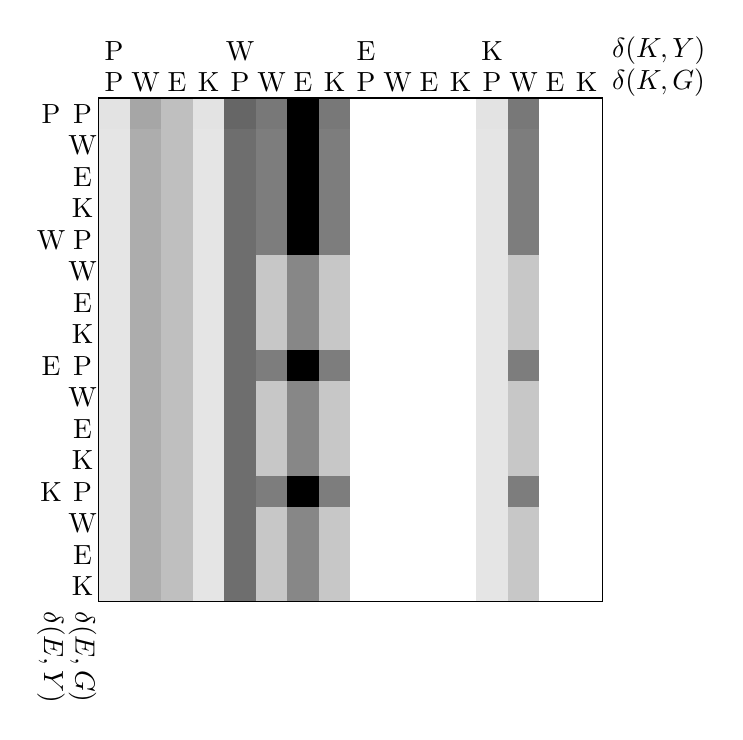
\begin{tikzpicture}[yscale=-1, scale=0.4]
  \node[anchor=west] at (16, -1.5) {$\delta (\q{K}, \q{Y})$};
  \node[anchor=west] at (16, -0.5) {$\delta (\q{K}, \q{G})$};
  \node[anchor=west, rotate=-90] at (-1.5, 16) {$\delta (\q{E}, \q{Y})$};
  \node[anchor=west, rotate=-90] at (-0.5, 16) {$\delta (\q{E}, \q{G})$};
  \node at (0.5, -1.5) {P}; \node at (-1.5, 0.5) {P};
  \node at (0.5, -0.5) {P}; \node at (-0.5, 0.5) {P};
  \node at (4.5, -0.5) {P}; \node at (-0.5, 4.5) {P};
  \node at (8.5, -0.5) {P}; \node at (-0.5, 8.5) {P};
  \node at (12.5, -0.5) {P}; \node at (-0.5, 12.5) {P};
  \node at (4.5, -1.5) {W}; \node at (-1.5, 4.5) {W};
  \node at (1.5, -0.5) {W}; \node at (-0.5, 1.5) {W};
  \node at (5.5, -0.5) {W}; \node at (-0.5, 5.5) {W};
  \node at (9.5, -0.5) {W}; \node at (-0.5, 9.5) {W};
  \node at (13.5, -0.5) {W}; \node at (-0.5, 13.5) {W};
  \node at (8.5, -1.5) {E}; \node at (-1.5, 8.5) {E};
  \node at (2.5, -0.5) {E}; \node at (-0.5, 2.5) {E};
  \node at (6.5, -0.5) {E}; \node at (-0.5, 6.5) {E};
  \node at (10.5, -0.5) {E}; \node at (-0.5, 10.5) {E};
  \node at (14.5, -0.5) {E}; \node at (-0.5, 14.5) {E};
  \node at (12.5, -1.5) {K}; \node at (-1.5, 12.5) {K};
  \node at (3.5, -0.5) {K}; \node at (-0.5, 3.5) {K};
  \node at (7.5, -0.5) {K}; \node at (-0.5, 7.5) {K};
  \node at (11.5, -0.5) {K}; \node at (-0.5, 11.5) {K};
  \node at (15.5, -0.5) {K}; \node at (-0.5, 15.5) {K};
  \fill[black!11!white] (0, 0) rectangle +(1, 1);
  \fill[black!10!white] (0, 1) rectangle +(1, 1);
  \fill[black!10!white] (0, 2) rectangle +(1, 1);
  \fill[black!10!white] (0, 3) rectangle +(1, 1);
  \fill[black!10!white] (0, 4) rectangle +(1, 1);
  \fill[black!10!white] (0, 5) rectangle +(1, 1);
  \fill[black!10!white] (0, 6) rectangle +(1, 1);
  \fill[black!10!white] (0, 7) rectangle +(1, 1);
  \fill[black!10!white] (0, 8) rectangle +(1, 1);
  \fill[black!10!white] (0, 9) rectangle +(1, 1);
  \fill[black!10!white] (0, 10) rectangle +(1, 1);
  \fill[black!10!white] (0, 11) rectangle +(1, 1);
  \fill[black!10!white] (0, 12) rectangle +(1, 1);
  \fill[black!10!white] (0, 13) rectangle +(1, 1);
  \fill[black!10!white] (0, 14) rectangle +(1, 1);
  \fill[black!10!white] (0, 15) rectangle +(1, 1);
  \fill[black!35!white] (1, 0) rectangle +(1, 1);
  \fill[black!32!white] (1, 1) rectangle +(1, 1);
  \fill[black!32!white] (1, 2) rectangle +(1, 1);
  \fill[black!32!white] (1, 3) rectangle +(1, 1);
  \fill[black!32!white] (1, 4) rectangle +(1, 1);
  \fill[black!32!white] (1, 5) rectangle +(1, 1);
  \fill[black!32!white] (1, 6) rectangle +(1, 1);
  \fill[black!32!white] (1, 7) rectangle +(1, 1);
  \fill[black!32!white] (1, 8) rectangle +(1, 1);
  \fill[black!32!white] (1, 9) rectangle +(1, 1);
  \fill[black!32!white] (1, 10) rectangle +(1, 1);
  \fill[black!32!white] (1, 11) rectangle +(1, 1);
  \fill[black!32!white] (1, 12) rectangle +(1, 1);
  \fill[black!32!white] (1, 13) rectangle +(1, 1);
  \fill[black!32!white] (1, 14) rectangle +(1, 1);
  \fill[black!32!white] (1, 15) rectangle +(1, 1);
  \fill[black!25!white] (2, 0) rectangle +(1, 1);
  \fill[black!25!white] (2, 1) rectangle +(1, 1);
  \fill[black!25!white] (2, 2) rectangle +(1, 1);
  \fill[black!25!white] (2, 3) rectangle +(1, 1);
  \fill[black!25!white] (2, 4) rectangle +(1, 1);
  \fill[black!25!white] (2, 5) rectangle +(1, 1);
  \fill[black!25!white] (2, 6) rectangle +(1, 1);
  \fill[black!25!white] (2, 7) rectangle +(1, 1);
  \fill[black!25!white] (2, 8) rectangle +(1, 1);
  \fill[black!25!white] (2, 9) rectangle +(1, 1);
  \fill[black!25!white] (2, 10) rectangle +(1, 1);
  \fill[black!25!white] (2, 11) rectangle +(1, 1);
  \fill[black!25!white] (2, 12) rectangle +(1, 1);
  \fill[black!25!white] (2, 13) rectangle +(1, 1);
  \fill[black!25!white] (2, 14) rectangle +(1, 1);
  \fill[black!25!white] (2, 15) rectangle +(1, 1);
  \fill[black!11!white] (3, 0) rectangle +(1, 1);
  \fill[black!10!white] (3, 1) rectangle +(1, 1);
  \fill[black!10!white] (3, 2) rectangle +(1, 1);
  \fill[black!10!white] (3, 3) rectangle +(1, 1);
  \fill[black!10!white] (3, 4) rectangle +(1, 1);
  \fill[black!10!white] (3, 5) rectangle +(1, 1);
  \fill[black!10!white] (3, 6) rectangle +(1, 1);
  \fill[black!10!white] (3, 7) rectangle +(1, 1);
  \fill[black!10!white] (3, 8) rectangle +(1, 1);
  \fill[black!10!white] (3, 9) rectangle +(1, 1);
  \fill[black!10!white] (3, 10) rectangle +(1, 1);
  \fill[black!10!white] (3, 11) rectangle +(1, 1);
  \fill[black!10!white] (3, 12) rectangle +(1, 1);
  \fill[black!10!white] (3, 13) rectangle +(1, 1);
  \fill[black!10!white] (3, 14) rectangle +(1, 1);
  \fill[black!10!white] (3, 15) rectangle +(1, 1);
  \fill[black!60!white] (4, 0) rectangle +(1, 1);
  \fill[black!57!white] (4, 1) rectangle +(1, 1);
  \fill[black!57!white] (4, 2) rectangle +(1, 1);
  \fill[black!57!white] (4, 3) rectangle +(1, 1);
  \fill[black!57!white] (4, 4) rectangle +(1, 1);
  \fill[black!57!white] (4, 5) rectangle +(1, 1);
  \fill[black!57!white] (4, 6) rectangle +(1, 1);
  \fill[black!57!white] (4, 7) rectangle +(1, 1);
  \fill[black!57!white] (4, 8) rectangle +(1, 1);
  \fill[black!57!white] (4, 9) rectangle +(1, 1);
  \fill[black!57!white] (4, 10) rectangle +(1, 1);
  \fill[black!57!white] (4, 11) rectangle +(1, 1);
  \fill[black!57!white] (4, 12) rectangle +(1, 1);
  \fill[black!57!white] (4, 13) rectangle +(1, 1);
  \fill[black!57!white] (4, 14) rectangle +(1, 1);
  \fill[black!57!white] (4, 15) rectangle +(1, 1);
  \fill[black!53!white] (5, 0) rectangle +(1, 1);
  \fill[black!51!white] (5, 1) rectangle +(1, 1);
  \fill[black!51!white] (5, 2) rectangle +(1, 1);
  \fill[black!51!white] (5, 3) rectangle +(1, 1);
  \fill[black!51!white] (5, 4) rectangle +(1, 1);
  \fill[black!22!white] (5, 5) rectangle +(1, 1);
  \fill[black!22!white] (5, 6) rectangle +(1, 1);
  \fill[black!22!white] (5, 7) rectangle +(1, 1);
  \fill[black!51!white] (5, 8) rectangle +(1, 1);
  \fill[black!22!white] (5, 9) rectangle +(1, 1);
  \fill[black!22!white] (5, 10) rectangle +(1, 1);
  \fill[black!22!white] (5, 11) rectangle +(1, 1);
  \fill[black!51!white] (5, 12) rectangle +(1, 1);
  \fill[black!22!white] (5, 13) rectangle +(1, 1);
  \fill[black!22!white] (5, 14) rectangle +(1, 1);
  \fill[black!22!white] (5, 15) rectangle +(1, 1);
  \fill[black!100!white] (6, 0) rectangle +(1, 1);
  \fill[black!100!white] (6, 1) rectangle +(1, 1);
  \fill[black!100!white] (6, 2) rectangle +(1, 1);
  \fill[black!100!white] (6, 3) rectangle +(1, 1);
  \fill[black!100!white] (6, 4) rectangle +(1, 1);
  \fill[black!47!white] (6, 5) rectangle +(1, 1);
  \fill[black!47!white] (6, 6) rectangle +(1, 1);
  \fill[black!47!white] (6, 7) rectangle +(1, 1);
  \fill[black!100!white] (6, 8) rectangle +(1, 1);
  \fill[black!47!white] (6, 9) rectangle +(1, 1);
  \fill[black!47!white] (6, 10) rectangle +(1, 1);
  \fill[black!47!white] (6, 11) rectangle +(1, 1);
  \fill[black!100!white] (6, 12) rectangle +(1, 1);
  \fill[black!47!white] (6, 13) rectangle +(1, 1);
  \fill[black!47!white] (6, 14) rectangle +(1, 1);
  \fill[black!47!white] (6, 15) rectangle +(1, 1);
  \fill[black!53!white] (7, 0) rectangle +(1, 1);
  \fill[black!51!white] (7, 1) rectangle +(1, 1);
  \fill[black!51!white] (7, 2) rectangle +(1, 1);
  \fill[black!51!white] (7, 3) rectangle +(1, 1);
  \fill[black!51!white] (7, 4) rectangle +(1, 1);
  \fill[black!22!white] (7, 5) rectangle +(1, 1);
  \fill[black!22!white] (7, 6) rectangle +(1, 1);
  \fill[black!22!white] (7, 7) rectangle +(1, 1);
  \fill[black!51!white] (7, 8) rectangle +(1, 1);
  \fill[black!22!white] (7, 9) rectangle +(1, 1);
  \fill[black!22!white] (7, 10) rectangle +(1, 1);
  \fill[black!22!white] (7, 11) rectangle +(1, 1);
  \fill[black!51!white] (7, 12) rectangle +(1, 1);
  \fill[black!22!white] (7, 13) rectangle +(1, 1);
  \fill[black!22!white] (7, 14) rectangle +(1, 1);
  \fill[black!22!white] (7, 15) rectangle +(1, 1);
  \fill[black!0!white] (8, 0) rectangle +(1, 1);
  \fill[black!0!white] (8, 1) rectangle +(1, 1);
  \fill[black!0!white] (8, 2) rectangle +(1, 1);
  \fill[black!0!white] (8, 3) rectangle +(1, 1);
  \fill[black!0!white] (8, 4) rectangle +(1, 1);
  \fill[black!0!white] (8, 5) rectangle +(1, 1);
  \fill[black!0!white] (8, 6) rectangle +(1, 1);
  \fill[black!0!white] (8, 7) rectangle +(1, 1);
  \fill[black!0!white] (8, 8) rectangle +(1, 1);
  \fill[black!0!white] (8, 9) rectangle +(1, 1);
  \fill[black!0!white] (8, 10) rectangle +(1, 1);
  \fill[black!0!white] (8, 11) rectangle +(1, 1);
  \fill[black!0!white] (8, 12) rectangle +(1, 1);
  \fill[black!0!white] (8, 13) rectangle +(1, 1);
  \fill[black!0!white] (8, 14) rectangle +(1, 1);
  \fill[black!0!white] (8, 15) rectangle +(1, 1);
  \fill[black!0!white] (9, 0) rectangle +(1, 1);
  \fill[black!0!white] (9, 1) rectangle +(1, 1);
  \fill[black!0!white] (9, 2) rectangle +(1, 1);
  \fill[black!0!white] (9, 3) rectangle +(1, 1);
  \fill[black!0!white] (9, 4) rectangle +(1, 1);
  \fill[black!0!white] (9, 5) rectangle +(1, 1);
  \fill[black!0!white] (9, 6) rectangle +(1, 1);
  \fill[black!0!white] (9, 7) rectangle +(1, 1);
  \fill[black!0!white] (9, 8) rectangle +(1, 1);
  \fill[black!0!white] (9, 9) rectangle +(1, 1);
  \fill[black!0!white] (9, 10) rectangle +(1, 1);
  \fill[black!0!white] (9, 11) rectangle +(1, 1);
  \fill[black!0!white] (9, 12) rectangle +(1, 1);
  \fill[black!0!white] (9, 13) rectangle +(1, 1);
  \fill[black!0!white] (9, 14) rectangle +(1, 1);
  \fill[black!0!white] (9, 15) rectangle +(1, 1);
  \fill[black!0!white] (10, 0) rectangle +(1, 1);
  \fill[black!0!white] (10, 1) rectangle +(1, 1);
  \fill[black!0!white] (10, 2) rectangle +(1, 1);
  \fill[black!0!white] (10, 3) rectangle +(1, 1);
  \fill[black!0!white] (10, 4) rectangle +(1, 1);
  \fill[black!0!white] (10, 5) rectangle +(1, 1);
  \fill[black!0!white] (10, 6) rectangle +(1, 1);
  \fill[black!0!white] (10, 7) rectangle +(1, 1);
  \fill[black!0!white] (10, 8) rectangle +(1, 1);
  \fill[black!0!white] (10, 9) rectangle +(1, 1);
  \fill[black!0!white] (10, 10) rectangle +(1, 1);
  \fill[black!0!white] (10, 11) rectangle +(1, 1);
  \fill[black!0!white] (10, 12) rectangle +(1, 1);
  \fill[black!0!white] (10, 13) rectangle +(1, 1);
  \fill[black!0!white] (10, 14) rectangle +(1, 1);
  \fill[black!0!white] (10, 15) rectangle +(1, 1);
  \fill[black!0!white] (11, 0) rectangle +(1, 1);
  \fill[black!0!white] (11, 1) rectangle +(1, 1);
  \fill[black!0!white] (11, 2) rectangle +(1, 1);
  \fill[black!0!white] (11, 3) rectangle +(1, 1);
  \fill[black!0!white] (11, 4) rectangle +(1, 1);
  \fill[black!0!white] (11, 5) rectangle +(1, 1);
  \fill[black!0!white] (11, 6) rectangle +(1, 1);
  \fill[black!0!white] (11, 7) rectangle +(1, 1);
  \fill[black!0!white] (11, 8) rectangle +(1, 1);
  \fill[black!0!white] (11, 9) rectangle +(1, 1);
  \fill[black!0!white] (11, 10) rectangle +(1, 1);
  \fill[black!0!white] (11, 11) rectangle +(1, 1);
  \fill[black!0!white] (11, 12) rectangle +(1, 1);
  \fill[black!0!white] (11, 13) rectangle +(1, 1);
  \fill[black!0!white] (11, 14) rectangle +(1, 1);
  \fill[black!0!white] (11, 15) rectangle +(1, 1);
  \fill[black!11!white] (12, 0) rectangle +(1, 1);
  \fill[black!10!white] (12, 1) rectangle +(1, 1);
  \fill[black!10!white] (12, 2) rectangle +(1, 1);
  \fill[black!10!white] (12, 3) rectangle +(1, 1);
  \fill[black!10!white] (12, 4) rectangle +(1, 1);
  \fill[black!10!white] (12, 5) rectangle +(1, 1);
  \fill[black!10!white] (12, 6) rectangle +(1, 1);
  \fill[black!10!white] (12, 7) rectangle +(1, 1);
  \fill[black!10!white] (12, 8) rectangle +(1, 1);
  \fill[black!10!white] (12, 9) rectangle +(1, 1);
  \fill[black!10!white] (12, 10) rectangle +(1, 1);
  \fill[black!10!white] (12, 11) rectangle +(1, 1);
  \fill[black!10!white] (12, 12) rectangle +(1, 1);
  \fill[black!10!white] (12, 13) rectangle +(1, 1);
  \fill[black!10!white] (12, 14) rectangle +(1, 1);
  \fill[black!10!white] (12, 15) rectangle +(1, 1);
  \fill[black!53!white] (13, 0) rectangle +(1, 1);
  \fill[black!51!white] (13, 1) rectangle +(1, 1);
  \fill[black!51!white] (13, 2) rectangle +(1, 1);
  \fill[black!51!white] (13, 3) rectangle +(1, 1);
  \fill[black!51!white] (13, 4) rectangle +(1, 1);
  \fill[black!22!white] (13, 5) rectangle +(1, 1);
  \fill[black!22!white] (13, 6) rectangle +(1, 1);
  \fill[black!22!white] (13, 7) rectangle +(1, 1);
  \fill[black!51!white] (13, 8) rectangle +(1, 1);
  \fill[black!22!white] (13, 9) rectangle +(1, 1);
  \fill[black!22!white] (13, 10) rectangle +(1, 1);
  \fill[black!22!white] (13, 11) rectangle +(1, 1);
  \fill[black!51!white] (13, 12) rectangle +(1, 1);
  \fill[black!22!white] (13, 13) rectangle +(1, 1);
  \fill[black!22!white] (13, 14) rectangle +(1, 1);
  \fill[black!22!white] (13, 15) rectangle +(1, 1);
  \fill[black!0!white] (14, 0) rectangle +(1, 1);
  \fill[black!0!white] (14, 1) rectangle +(1, 1);
  \fill[black!0!white] (14, 2) rectangle +(1, 1);
  \fill[black!0!white] (14, 3) rectangle +(1, 1);
  \fill[black!0!white] (14, 4) rectangle +(1, 1);
  \fill[black!0!white] (14, 5) rectangle +(1, 1);
  \fill[black!0!white] (14, 6) rectangle +(1, 1);
  \fill[black!0!white] (14, 7) rectangle +(1, 1);
  \fill[black!0!white] (14, 8) rectangle +(1, 1);
  \fill[black!0!white] (14, 9) rectangle +(1, 1);
  \fill[black!0!white] (14, 10) rectangle +(1, 1);
  \fill[black!0!white] (14, 11) rectangle +(1, 1);
  \fill[black!0!white] (14, 12) rectangle +(1, 1);
  \fill[black!0!white] (14, 13) rectangle +(1, 1);
  \fill[black!0!white] (14, 14) rectangle +(1, 1);
  \fill[black!0!white] (14, 15) rectangle +(1, 1);
  \fill[black!0!white] (15, 0) rectangle +(1, 1);
  \fill[black!0!white] (15, 1) rectangle +(1, 1);
  \fill[black!0!white] (15, 2) rectangle +(1, 1);
  \fill[black!0!white] (15, 3) rectangle +(1, 1);
  \fill[black!0!white] (15, 4) rectangle +(1, 1);
  \fill[black!0!white] (15, 5) rectangle +(1, 1);
  \fill[black!0!white] (15, 6) rectangle +(1, 1);
  \fill[black!0!white] (15, 7) rectangle +(1, 1);
  \fill[black!0!white] (15, 8) rectangle +(1, 1);
  \fill[black!0!white] (15, 9) rectangle +(1, 1);
  \fill[black!0!white] (15, 10) rectangle +(1, 1);
  \fill[black!0!white] (15, 11) rectangle +(1, 1);
  \fill[black!0!white] (15, 12) rectangle +(1, 1);
  \fill[black!0!white] (15, 13) rectangle +(1, 1);
  \fill[black!0!white] (15, 14) rectangle +(1, 1);
  \fill[black!0!white] (15, 15) rectangle +(1, 1);
  \draw (0, 0) rectangle (16, 16);
\end{tikzpicture}
  \end{center}
  \caption{A heatmap of the distribution of unique machines after renaming states.}
  \label{fig:rename}
\end{figure}

\section{DFA minimisation}

One form of redundancy which dead code elimination cannot identify
is when two states have the same effects. Consider the
(part of a) machine in Figure~\ref{fig:equivalent-states} for example:
intuitively the machine always keeps the board unchanged, and
always moves towards the Ghost Gum tree. More formally, its two states
are equivalent, as outgoing transitions from the states have the same effects,
and the outgoing transitions target states which are equivalent, so
the states can be merged as in Figure~\ref{fig:normalised-states}. Dead
code elimination cannot normalise this machine further, as both states
are live. Renaming could only normalise the mirror image of the former
machine to the former machine.

\begin{figure}
  \begin{subfigure}[b]{0.5\textwidth}
    \begin{center}
      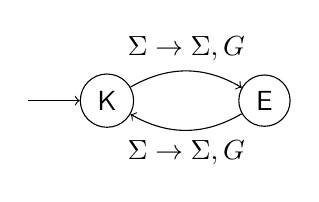
\begin{tikzpicture}
        \node[draw,circle](K) at (0, 0) {\sffamily K};
        \node[draw,circle](E) at (2, 0) {\sffamily E};
        \draw[->] (-1, 0) -- (K);
        \path[->] (K) edge[bend left]
        node[pos=0.5, above] {$\Sigma \rightarrow \Sigma, \q{G}$}
        (E);
        \path[->] (E) edge[bend left]
        node[pos=0.5, below] {$\Sigma \rightarrow \Sigma, \q{G}$}
        (K);
      \end{tikzpicture}
    \end{center}
    \caption{Before normalisation.}
    \label{fig:equivalent-states}
  \end{subfigure}
  \begin{subfigure}[b]{0.5\textwidth}
    \begin{center}
      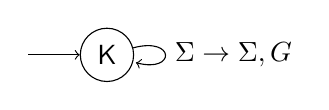
\begin{tikzpicture}
        \node[draw,circle](K) at (0, 0) {\sffamily K};
        \draw[->] (-1, 0) -- (K);
        \path[->] (K) edge[loop right]
        node[pos=0.5, right] {$\Sigma \rightarrow \Sigma, \q{G}$}
        (K);
      \end{tikzpicture}
    \end{center}
    \caption{After normalisation.}
    \label{fig:normalised-states}
  \end{subfigure}
  \caption{A machine with two equivalent states.}
\end{figure}

\subsection{Extending DFA minimisation}

An algorithm for minimising discrete finite automata (DFAs) can
identify a similar redundancy in DFAs. Baumann
\cite{baumann} extends Hopcroft's algorithm \cite{hopcroft} to identify
redundant states in \emph{Mealy~machines} \cite{mealy}, by requiring
that transitions must also produce the same outputs in order to be
equivalent. I treat Platypus machines as Mealy machines, with the
output of each transition being the direction to move and the colour
to write of the transition, i.e. the action on the board. This \emph{abstraction}
applied to a Turing machine is depicted in Figure~\ref{fig:mealy}.

\begin{figure}
  \begin{center}
    \begin{tikzpicture}
      % Mealy machine
      \node[draw,circle](A) at (0.0, 0.5) {};
      \node[draw,circle](B) at (1, 1) {};
      \node[fill,gray, circle](C) at (0.8, 0) {};
      \node[draw,circle] at (0.8, 0) {}; % outline for C
      \draw[->] (A) -- (B);
      \draw[->] (B) -- (C);
      \draw[->] (C) -- (A);
      \node[draw, fit=(A) (B) (C), inner sep=1ex] (Mealy) {};
      \node[above=0ex of Mealy] {Machine};

      \node[draw, inner sep=1ex](Tape) at (-3, 0.5) {
        $\begin{array}{c}
            \vdots \\ \q{Y} \\ \q{G} \\ \fbox{$\q{G}$} \\ \q{Y} \\ \vdots
         \end{array}$
      };
      \node[above=0ex of Tape] {Tape};
      \draw[transform canvas={yshift=1em}, ->] (Mealy) -- (Tape) node[pos=0.5, above] {$\Sigma, \{\q{L}, \q{R}\}$};
      \draw[transform canvas={yshift=-1em}, ->] (Tape) -- (Mealy) node[midway, below] {$\Sigma$};
    \end{tikzpicture}
  \end{center}
  
  \caption{A Turing machine may be abstracted as a Mealy machine.}
  \label{fig:mealy}
\end{figure}

This abstraction may seem odd, as a Turing machine is
more powerful than a Mealy machine. But a result of the abstraction
is that the minimisation algorithm only now does not model the state
of the tape at all, providing a conservative and sound approximation of
the Turing machine. The tape only ensures that that some particular
sequences of outputs may prevent the machine from receiving
some sequences of inputs; an equivalence algorithm for Mealy
machines is unaware of this constraint, and thus an equivalence
algorithm only considers execution paths which can never occur. For
example, if a Turing machine writes a symbol to a cell then immediately
reads the same cell, the machine can only read that symbol again; but an
equivalence algorithm will needlessly consider what would occur if the
machine reads any symbol. Thus the algorithm is conservative but safe --
it may unnecessarily split equivalence classes, but the abstraction will
not cause the algorithm to unsoundly merge equivalence classes.

But we cannot trust the state of a Platypus board when reasoning
about one Platypus machine anyway, as the opponent of a machine may
(more or less) arbitrarily modify the board, invalidating any assumptions
about the state of the board. For example, a machine which always fills
the board with Yellow is not distinguishable from a machine which
always preserves the state of the board, if only that one machine uses the board.
(Recall that the board is initially all Yellow.) Introducing another
machine which concurrently fills the board with Green provokes
different behaviour out of the Yellow-filling and board-preserving
machines, and so they are not equivalent.

Also note that states must be partitioned by the number of outgoing
transitions, as Platypus machines are incomplete by definition. Thus
the minimisation algorithm begins with the equivalence sets
$\setb{\setb{\q{Platypus}}, \setb{\q{Wombat}, \q{Emu}, \q{Kangaroo}}}$.

\subsection{Implementation}

I implemented a fast version of Nerode's algorithm for minimising
DFAs \cite{nerode}. Though the algorithm has worse complexity
($\mathcal{O}(n^2)$ for $n$ states) than Hopcroft's algorithm
($\mathcal{O}(n \log n)$) the number of states is small, allowing for
constant factors to have large influence on performance, and the
algorithm lends itself to data parallelism with a
\emph{single instruction-multiple data} (SIMD) implementation.

In essence the algorithm iteratively constructs an array containing
which denotes pairs of states which are distinguishable. Let $A$ be
this array, where $A_{a, b}$ denotes that the states $a$ and $b$ may
be distinguished. $A$ is symmetric, i.e.
$ \forall a, b\ldotp A_{a, b} = A_{b, a} $. Initially $A_{a, b}$ is set to
if $a$ and $b$ have a different number of outgoing
states, or the transitions leaving $a$ and $b$ have different effects.
Then the array is iterated by marking states as distinct when they
have transitions which lead to distinct states. The algorithm
terminates when no elements of $A$ are changed.
Each state $S$ is then renamed to the highest-numbered state that
is not distinct from $S$ according to $A$. This renaming notably
preserves the Platypus state, as no other states will ever be equivalent
to the Platypus state, and the algorithm preserves the Kangaroo state,
as it has the greatest index per the representation in Section~\ref{sec:representation}.

As forementioned the algorithm can be implemented with data parallelism.
The SIMD extensions for x86 beginning with the \emph{Streaming SIMD Extensions} (SSE)
offer operations which perform an operation on each of 16 byte-sized \emph{lanes}
at once, which allows the entirety of $A$ to be updated in parallel, if each
element is stored as one byte.\footnote{Note that $A$ is two-dimensional, but
  a vector is one-dimensional, so the implementation must convert
  two-dimensional indices to one-dimensional indices. I chose to use
  \emph{row-major order} to be consistent with arrays in Common Lisp, but
  this decision is arbitrary and does not affect the behaviour of the algorithm.}
The most difficult part of a SIMD implementation
is following transitions, which require two particular permutations of the lanes
to compute derivatives, and then an arbitrary permutation in order to index $A$
with the derivatives. Fortunately, there is an operation to perform an arbitrary
permutation, namely the \emph{shuffle} operation\footnote{Although the \texttt{pshufb}
  instruction was only introduced in the \emph{Supplemental Streaming SIMD
    Extensions 3} (SSSE3) instruction set. I envy the person who gets to come up with
  these names.};
its use follows the approach Geoff Langdale used for implementing discrete finite
automata with SIMD code \cite{sheng,hyperscan}. The algorithm is presented in
Figure~\ref{fig:nerode}, though for \emph{complete} Mealy machines to simplify
presentation. The algorithm must treat undefined transitions as distinct from
any defined transition in order to handle \emph{incomplete} machines; for
example, such treatment must be given for reading a Green cell from the Platypus
state with a Platypus machine.

\begin{figure}
  \begin{center}
    \begin{tabular}{l}
      \emph{Set up initial state and target lookup table} \\
      \textbf{for each state} a, b, \textbf{each symbol} s \\
      \quad distinct[states $\times$ a + b] $\leftarrow$ output(a, s) $\neq$ output(b, s) \\
      \textbf{for each state} q, \textbf{each symbol} s \\
      \quad target[symbols $\times$ q + s] = target(q, s) \\
      rows = row indices \\
      cols = column indices \\
      \emph{Row-major access functions} \\
      A(a, b) = shuffle(vector: distinct, indices: states $\times$ a + b) \\
      out(q, s) = shuffle(vector: target, indices: symbols $\times$ q + s) \\
      \emph{Iterate} \\
      \textbf{while} distinct \textbf{changes} \\
      \quad \textbf{for each symbol} s \\
      \quad\quad distinct $\leftarrow$ distinct $\lor$ A(target(rows, s), target(columns, s))
    \end{tabular}
  \end{center}
  \caption{Iterating Nerode's algorithm with SIMD code.}
  \label{fig:nerode}
\end{figure}

I have yet to analyse the complexity of the parallel algorithm, but its
\emph{depth} must be in $\mathcal{O}(n^2)$, as at worst the algorithm
can only avoid termination by updating two elements (due to symmetry)
of the $n^2$ elements of $A$ which was previously false.
In practice processing every Platypus machine requires very few
iterations; 227 million machines require just one iteration, 41 million
require two iterations, and 602 thousand require three.

The algorithm may be extended to larger machines
(such as busy beaver machines) when larger SIMD operations are
available. The AVX-512 extension provides instructions
which work in parallel over 64 bytes for example, allowing for the
minimisation of 8-state machines. The \emph{Neon} extension for
ARM includes a \texttt{tbl} instruction which can shuffle from a 64
byte table, despite Neon only providing 16 byte operations otherwise;
the other operations would have to be performed four times.

107,452,240 unique machines (40.03\%) remain after minimisation.
This is only barely better than dead code elimination, and much
worse than renaming, as minimisation cannot detect mirror images.
Performing renaming after minimisation yields a similarly slight
improvement with 53,726,320 unique machines (20.01\%) remaining. The
results of the combined algorithms are not visually distinguishable from
the results of renaming alone, though it eliminates 83.1 trillion matches
from the Platypus tournament due to the quadratic time complexity of
the tournament. It took 359 CPU-seconds to perform minimisation and
renaming of all Platypus machines.

\section{Differential testing}

I have argued that the proposed algorithms are sound, but bugs may still arise
in the implementation of these algorithms. The implementations of the
algorithms are concise: DCE and renaming are implemented each with
less than 30 lines of code, and DFA minimisation consists of 52 lines of code%
\footnote{This figure does not include the 40 lines of code used to manipulate
  the representation of Platypus machines. The functions manipulating the
  representation are trivial, performing no mutation and minimal
  control flow, and may be tested independently, so I am less concerned about
  bugs in the representation.}, so it is feasible to manually inspect the
implementations. I used \emph{differential testing} to try to find cases where
normalisation does not produce an equivalent machine to be safe. The testing
program generates two random machines and asserts that normalisation
does not change the outcome of a match between the machines, i.e.

$$\forall m, n\ldotp \q{run}(m, n) = \q{run}(\q{normalise}(m), n) = \q{run}(m, \q{normalise}(n))$$

The testing program initially detected a bug in the Platypus game interpreter,
which managed to incorrectly decode a machine, leading to deviations
between a machine and normalisation of the machine. Dead code elimination
and renaming were tested for 30 billion games each, without finding any errors.
The testing program was also instrumental in finding several bugs in the
implementation of DFA minimisation.

\section{Heuristics}

It may be the case that few equivalence sets cover most of the machines,
and so approximate results can be found by running just those
equivalence sets. Figure~\ref{fig:coverage} shows the coverage produced by
combined DFA minimisation and renaming; a mere 1\% of the equivalence
sets cover over 55\% of the machines, but coverage only increases linearly
past a few percent. Almost all equivalence sets only contain two machines,
as every machine has a mirror image. While the coverage of so few equivalence
sets is interesting, it is still too small to produce useful approximations in
my opinion.

\begin{figure}
  \centering
  \begin{tikzpicture}
    \begin{axis}[
      xlabel=Proportion of sets covered,
      ylabel=Proportion of machines covered,
      width=0.8\textwidth, height=8cm]
      \addplot[mark=none] table[x=amount, y=density, col sep=comma] {early-stopping.csv};
    \end{axis}
  \end{tikzpicture}
  \caption{The machines covered by testing varying amounts of equivalence sets.}
  \label{fig:coverage}
\end{figure}